\documentclass[uplatex, a4paper, 12pt, openany, oneside]{jsbook}

\usepackage[dvipdfmx]{graphicx}
\usepackage[dvipdfmx]{color}
\usepackage[dvipdfmx, bookmarks=true, setpagesize=false, hidelinks]{hyperref}
\usepackage{pxjahyper}

\usepackage{thesis}
\usepackage{here}
\usepackage{url}
\usepackage{amsmath} % 数式


\thesis{卒 業 論 文}
\title{
  \centering
    \scalebox{1.0}{モデル予測制御による二足歩行ロボットの歩行パターン生成}\\
    \scalebox{1.0}{ーパラメータに関する考察ー}\\
    \vspace{-0.3zh}
    \scalebox{0.65}{A walking pattern generation
    for biped robots using model predictive control}
    \scalebox{0.7}{- Consideration of parameters -}
    \vspace{-0.6zh}
}
\setlength{\textwidth}{\fullwidth}
\setlength{\evensidemargin}{\oddsidemargin}

\date{\today}
\vspace{-15.0zh}
\teacher{林原 靖男 教授}
\vspace{-15.0zh}
\organization{千葉工業大学 先進工学部 未来ロボティクス学科}
\author{20C1028 小川晴生}
\vspace{-15zh}

\renewcommand{\baselinestretch}{1.2}
\begin{document}

%% Front Matter
\frontmatter{}
%
\include{frontmatter/main}
%
%% Main Matter
\mainmatter{}
%
\include{introduction/main}
%ここにディレクトリのパスを追加していく
% 第2章
\chapter{MPCによる歩行パターン生成}
\section{緒言}
 本章では二足歩行ロボットの歩行パターン生成に関する基本的な概念,及び提案手法について述べる.

\section{歩行(walk)}


\section{ZMP}
 二足歩行ロボットの安定性判別の指標として代表的なものとして, Vukobratović らによって提案された Zero Moment Point (以下, ZMP ) [1] がある. 以下の図\ref{Fig:Definition of Zero-Moment Point}はロボットの足部における力の分布例である.足部の境界の内側に存在する点に作用する等価な力Rとしてまとめられる.力ベクトルRが通過するこの作用点がZMPの位置である.


\begin{figure}[H]
  \centering
 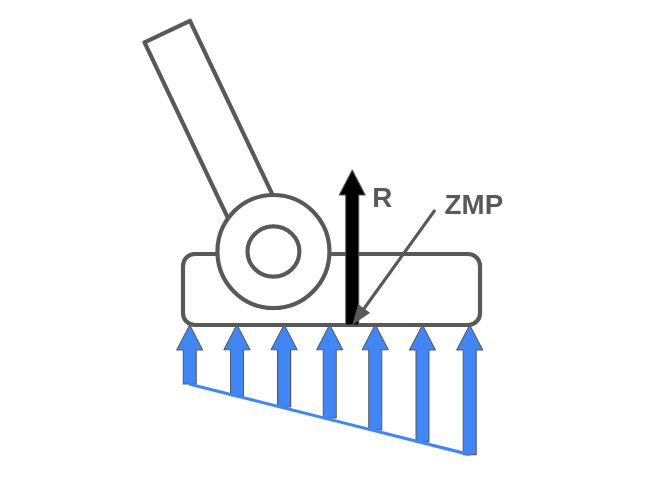
\includegraphics[keepaspectratio, scale=0.4]
      {images/walk/zmp.png}
 \caption{Definition of Zero-Moment Point}
 \label{Fig:Definition of Zero-Moment Point}
\end{figure}

 ZMPと関連する概念として支持多角形がある.
図に示すようにロボットが床面に接触している点で囲った範囲を支持多角形と考える.
この範囲に重心位置及びZMPがあれば,静的安定であり転倒しない.ZMPは常に支持多角形の中に存在する関係である.

\begin{figure}[H]
     \centering
    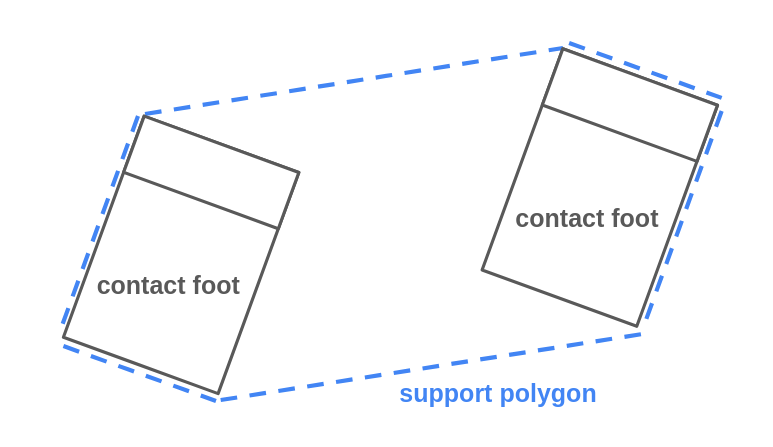
\includegraphics[keepaspectratio, scale=0.4]
         {images/walk/support_polygon.png}
    \caption{Support Polygon}
    \label{Fig:Support Polygon}
\end{figure}

%---------------------------------------
\section{テーブル台車モデル(Table-cart model)}
二足歩行ロボットのモデル化手法として,図\ref{Fig:Illustration of Table-cart model}に示すようなテーブル・台車モデルがある.質量の無視できるテーブルの上に質量Mをもつ台車が水平に走行できると考える.テーブルの台座が台車の走行範囲に比べて狭いため,台車がテーブルの端に達すると全体が転倒してしまうが,台車が適切な加速を行えば転倒を防ぐことができる.\\
このモデルから式(\ref{eq:zmp})のダイナミクスを導ける.ここでは,$x$, $\ddot{x}$はロボットの重心位置と重心加速度,$hCoM$は鉛直方向の重心の高さ,$g$は重力加速度,$p$はZMPの位置である.式(\ref{eq:zmp})によるモデル化に対し,システムへの入力を台車の重心の躍度(jerk),$\dddot{x}$とおくと,式(\ref{eq:system1}),式(\ref{eq:system2})のようなシステムとして表現できる.

%テーブル台車では重心の運動によってZMPが発生する因果関係を前提とすると,目標とするZMP軌道を定めてからこれを実現する安定な重心運動を計算する手順の歩行パターンの手法をZMPを規範とする歩行パターン生成法という.

\begin{equation}
     p=x-\frac{h_{CoM}}{g}\ \ddot{x}
     \label{eq:zmp}
\end{equation}

\begin{equation}
     \frac{d}{dt}\left(\begin{matrix}x\\\dot{x}\\\ddot{x}\\\end{matrix}\right)=\left(\begin{matrix}0&1&0\\0&0&1\\0&0&0\\\end{matrix}\right)\left(\begin{matrix}x\\\dot{x}\\\ddot{x}\\\end{matrix}\right)+\left(\begin{matrix}0\\0\\1\\\end{matrix}\right)u
     \label{eq:system1}
\end{equation}

\begin{equation}
     p=\left(\begin{matrix}1&0&-\frac{h_{CoM}}{g}\ \\\end{matrix}\right)\left(\begin{matrix}x\\\dot{x}\\\ddot{x}\\\end{matrix}\right)
     \label{eq:system2}
\end{equation}

ここで,上記のシステムを離散化すると,システムは式(\ref{eq:2.4})\~{}(\ref{eq:2.6})で表すことができる.

\begin{equation}
     \widehat{x}_k=\left(\begin{matrix}x\left(kT\right)\\\dot{x}\left(kT\right)\\\ddot{x}\left(kT\right)\\\end{matrix}\right),u_k=\dddot{x}\left(kT\right),z_k=z\left(kT\right)
     \label{eq:2.4}
\end{equation}

\begin{equation}
     \widehat{x}_{k+1}=\left(\begin{matrix}1&T&T^2/2\\0&1&T\\0&0&1\\\end{matrix}\right)\widehat{x}_k+\left(\begin{matrix}T^3/6\\T^3/2\\T\\\end{matrix}\right)u_k
     \label{eq:2.5}
\end{equation}

\begin{equation}
     z_k=\left(\begin{matrix}1&0&-\frac{h_{CoM}}{g}\ \\\end{matrix}\right)\widehat{x}_k
     \label{eq:2.6}
\end{equation}

\begin{figure}[H]
  \centering
 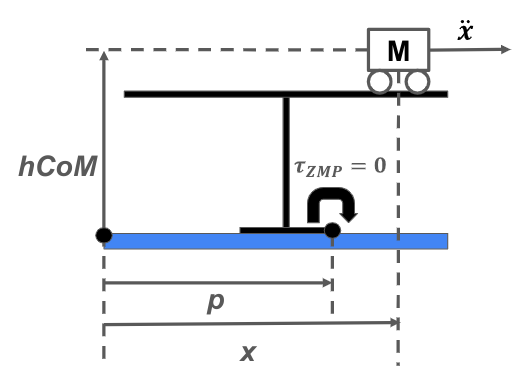
\includegraphics[keepaspectratio, scale=0.5]
      {images/walk/table.png}
 \caption{Illustration of Table-cart model}
 \label{Fig:Illustration of Table-cart model}
\end{figure}

% -----------------------------------------------------------
\section{予見制御による歩行パターン生成手法}
上記の ZMP とテーブル台車モデルの概念を利用した歩行パターン生成手法としては,kajita らによる予見制御を利用した歩行パターン生成手法 [2] がある. kajita らによる手法では (2.4)˜(2.6) で表現したロボットのダイナミクスに対して,予見制御理論によって以下の評価関数式 (2.7) を最小化する制御入力(二足歩行ロボットの歩行パターン)を得る.


\begin{equation}
     \min_{\substack{{\dddot{x}}_k,\ {\dddot{x}}_{k+1},\ \cdots}} \sum_{i=k}^{\infty}\left(\frac{1}{2}Q\left(z_{i+1}-z_{i+1}^{ref}\right)^2\ +\ \frac{1}{2}R{\dddot{x}}_i^2\right)
\end{equation}


式 (2.7) 内, z は ZMP の位置, z ref は ZMP の目標位置, u は入力である重心の躍度( jerk ),Q と R は重みを示す.
%---------------------------------------------------------------
\section{MPCを利用した歩行パターン生成手法}
本研究では, kajita らによる予見制御を利用した歩行パターン生成手法 [2] を MPC によって拡張した, Wieber らによる手法 [3] を実装する.ここでは,その手法 [3] について紹介する.
まず, MPC は最適制御の一種であり,無限長の区間に渡る最適化問題を解く代わりに,有限長の区間で最適化問題を解いて最適入力を得る手法である.有限区間の最適化問題であるがゆえに,陽に表現した制約を考慮しながら最適化問題を解くことができるのが特徴である.また,有限区間での最適化問題を解く際には,有限区間に渡る未来の状態,ないしは出力の予測値を利用して最適化を行う.式 (2.8) で表されるダイナミクスからなる一般的なシステムでは,状態の予測は式 (2.9) で表される

\begin{equation}
     \left\{\begin{aligned}\dot{x} &= Ax + Bu \\ y &= Cx \\\end{aligned}\right.
\end{equation}

\begin{equation}
     \left(\begin{matrix}x_{k+1}\\x_{k+2}\\x_{k+3}\\\vdots\\x_{k+n}\\\end{matrix}\right)=\left(\begin{matrix}A\\A^2\\A^3\\\vdots\\A^n\\\end{matrix}\right)x_k+\left(\begin{matrix}B&0&\cdots&&0\\AB&B&0&\cdots&0\\A^2&AB&B&\cdots&0\\\vdots&\vdots&&&0\\A^{n-1}B&A^{n-2}B&\cdots&AB&B\\\end{matrix}\right)\left(\begin{matrix}u_k\\u_{k+1}\\u_{k+2}\\\vdots\\u_{k+n-1}\\\end{matrix}\right)
\end{equation}

\begin{equation}
     C=\left(\begin{matrix}C&0&\cdots&0\\0&C&\cdots&0\\\vdots&&\ddots&0\\0&\cdots&&C\\\end{matrix}\right)
\end{equation}

\begin{equation}
     \left(\begin{matrix}z_{k+1}\\z_{k+2}\\z_{k+3}\\\vdots\\z_{k+n}\\\end{matrix}\right)=\left(\begin{matrix}C&0&\cdots&0\\0&C&\cdots&0\\\vdots&&\ddots&0\\0&\cdots&&C\\\end{matrix}\right)\left(\begin{matrix}x_k\\x_{k+1}\\x_{k+2}\\\vdots\\x_{k+n-1}\\\end{matrix}\right)
\end{equation}

\begin{equation}
     \min_{\substack{{\dddot{x}}_k,\ {\dddot{x}}_{k+1},\ \cdots,\ {\dddot{x}}_{k+n}}} \sum_{i=k}^{n}\left(\frac{1}{2}Q\left(z_{i+1}-z_{i+1}^{ref}\right)^2\ +\ \frac{1}{2}R{\dddot{x}}_i^2\right)
\end{equation}

\begin{equation}
     \left(\begin{matrix}L_{u_0}\\\vdots\\L_{u_n}\\\end{matrix}\right)\le\dddot{x}\le\left(\begin{matrix}U_{u_0}\\\vdots\\U_{u_n}\\\end{matrix}\right)
\end{equation}

\begin{equation}
     \left(\begin{matrix}L_{x_0}\\\vdots\\L_{x_n}\\\end{matrix}\right)\le z\le\left(\begin{matrix}U_{x_0}\\\vdots\\U_{x_n}\\\end{matrix}\right)
\end{equation}

\newpage

% 第3章
\chapter{実験環境}
 本章では,本研究で使用する歩行パターン生成器の説明及び実験環境やパラメータについて述べる.
本章では,本研究で行う実験に用いる実験環境や歩行パターン生成器について述べる.

\section{実験装置}
実験装置を表\ref{tab:Experimental Setup}に示す.また,本研究で使用する歩行パターン生成器は図のものである.はC++言語で実装されているMPCによる歩行パターン生成器である.表に示すライブラリ群を利用する.
\begin{table}[H]
  \centering
  \caption{Experimental Setup}
  \label{tab:Experimental Setup}
  \begin{tabular}{|l|l|}
      \hline \hline
       Device    & MacBook Air \\ \hline
       CPU       & Intel® Core™ i5-5250U CPU @ 1.60GHz × 4 \\ \hline
       RAM       & 7.7 GiB \\ \hline
       OS        & Ubuntu 20.04.6 LTS \\ \hline
  \end{tabular}
\end{table}

\begin{table}[H]
  \centering
  \caption{Libraries}
  \label{tab:Libraries}
  \begin{tabular}{|c|c|}
       \hline \hline
       QP solver                & osqp                  \\ \hline
       C++ binding of osqp      & osqp-eigen            \\ \hline
       Linear algebra library   & eigen-3.4.0           \\ \hline
  \end{tabular}
\end{table}

\begin{figure}[H]
  \centering
 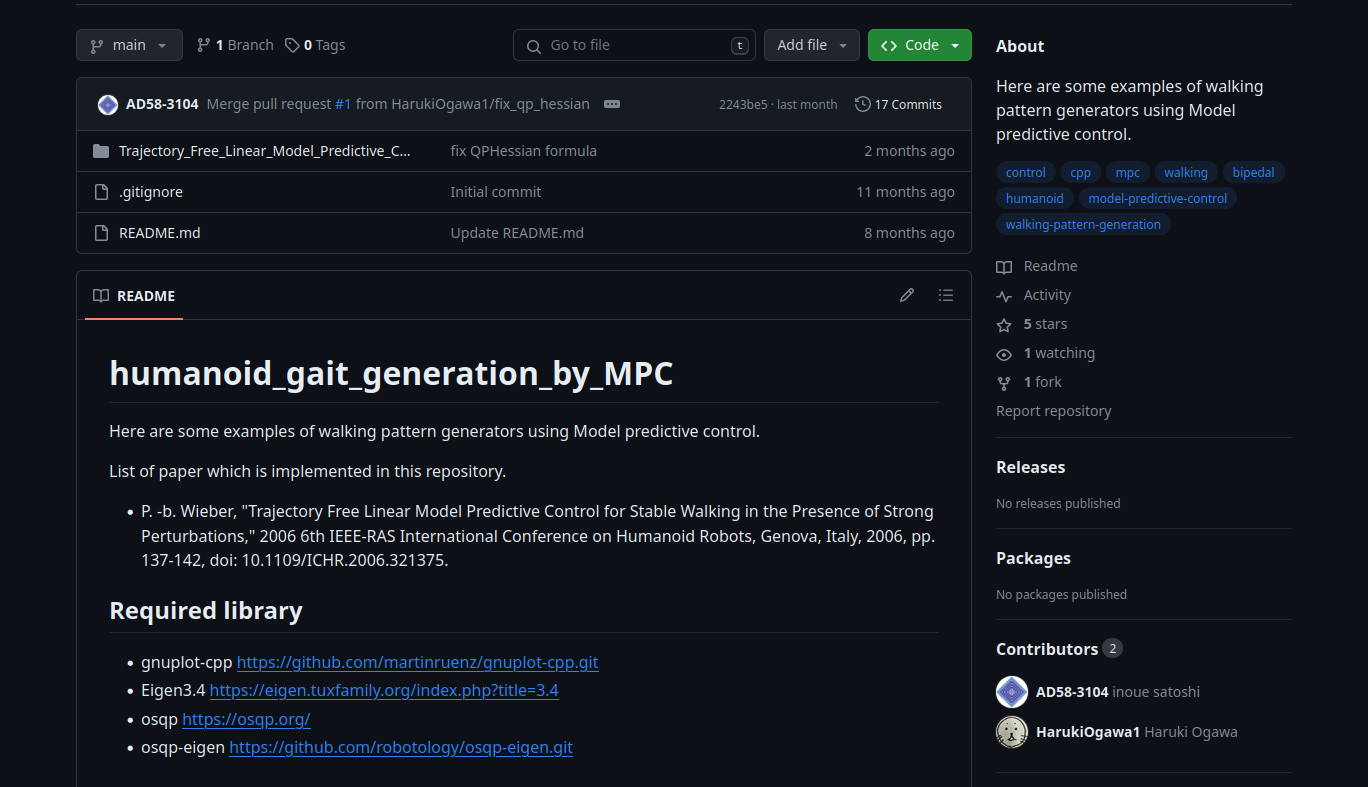
\includegraphics[keepaspectratio, scale=0.3]
      {images/github.png}
 \caption{GitHub page of publication}
 \label{Fig:GitHub page of publication}
\end{figure}


\section{本研究の歩行パターン生成器のパラメータ}
ここでは,4章に示す歩行パターンを生成可能なパラメータについて解説する.


\begin{table}[H]
  \centering
  \caption{Libraries used for implementation}
  \label{Libraries used for implementation}
  \begin{tabular}{|c|r|}
       \hline \hline
       Control Horizon                                          & 1.5{[}s{]}                      \\ \hline
       Unit time                                                & 10{[}s{]}                       \\ \hline
       Q / R                                                    & 1000000.0                        \\ \hline
       Height of CoM                                            & 0.6{[}m{]}                      \\ \hline
       Step width                                               & 0.15{[}m{]}                     \\ \hline
       start\_with\_this\_step                                  & 0.8{[}s{]}                      \\ \hline
       cycle\_step                                              & 0.4{[}s{]}                      \\ \hline
       double\_support\_step                                    & 0.1{[}s{]}                      \\ \hline \hline
       Upper bound of difference between ref and current output & 0.02{[}m{]}                     \\ \hline
       Lower bound of difference between ref and current output & -0.02{[}m{]}                    \\ \hline
       Upper bound of input                                     & 100{[}m/s\textsuperscript{3}{]} \\ \hline
       Lower bound of input                                     & 100{[}m/s\textsuperscript{3}{]} \\ \hline
  \end{tabular}
\end{table}

\begin{figure}[H]
  \centering
 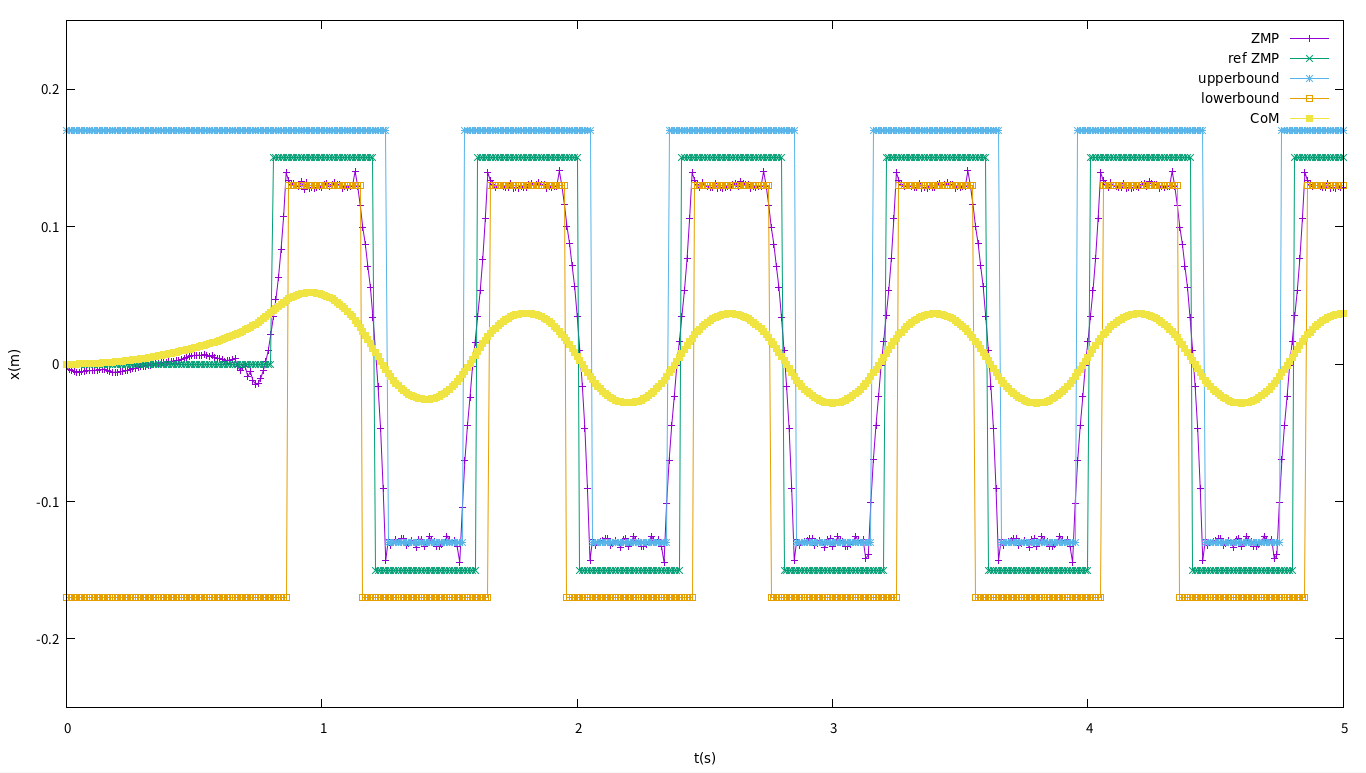
\includegraphics[keepaspectratio, scale=0.3]
      {images/mpc_sample.png}
 \caption{例になる歩行パターン}
 \label{Fig:例になる歩行パターン}
\end{figure}


\newpage

% 第3章
\chapter{パラメータに関する考察}
\section{実験目的}
本章では,二足歩行ロボットの歩行パターン生成のパラメータによって波形にどのような影響を与えているかを検証する.
検証するパラメータはControl Horizon,Q / R,start with this stepである.また,各パラメータごとに実行時間を記録する.

\section{実験結果}

\subsection{Control Horizon}
\begin{figure}[H]
  \centering
 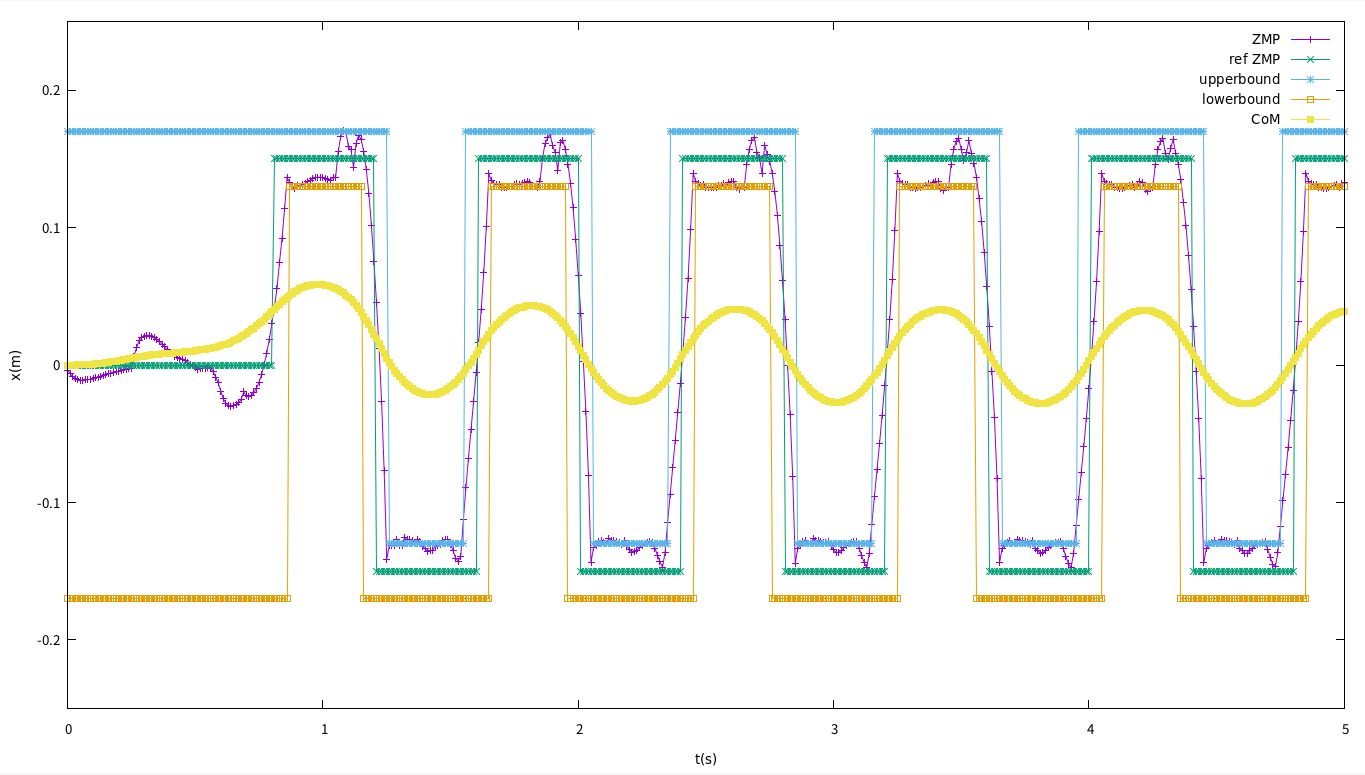
\includegraphics[keepaspectratio, scale=0.25]
      {images/mpc_horizon/mpc_horizon_100.png}
 \caption{Illustration of table-cart model}
 \label{Fig:Illustration of table-cart model}
\end{figure}

\begin{figure}[H]
  \centering
 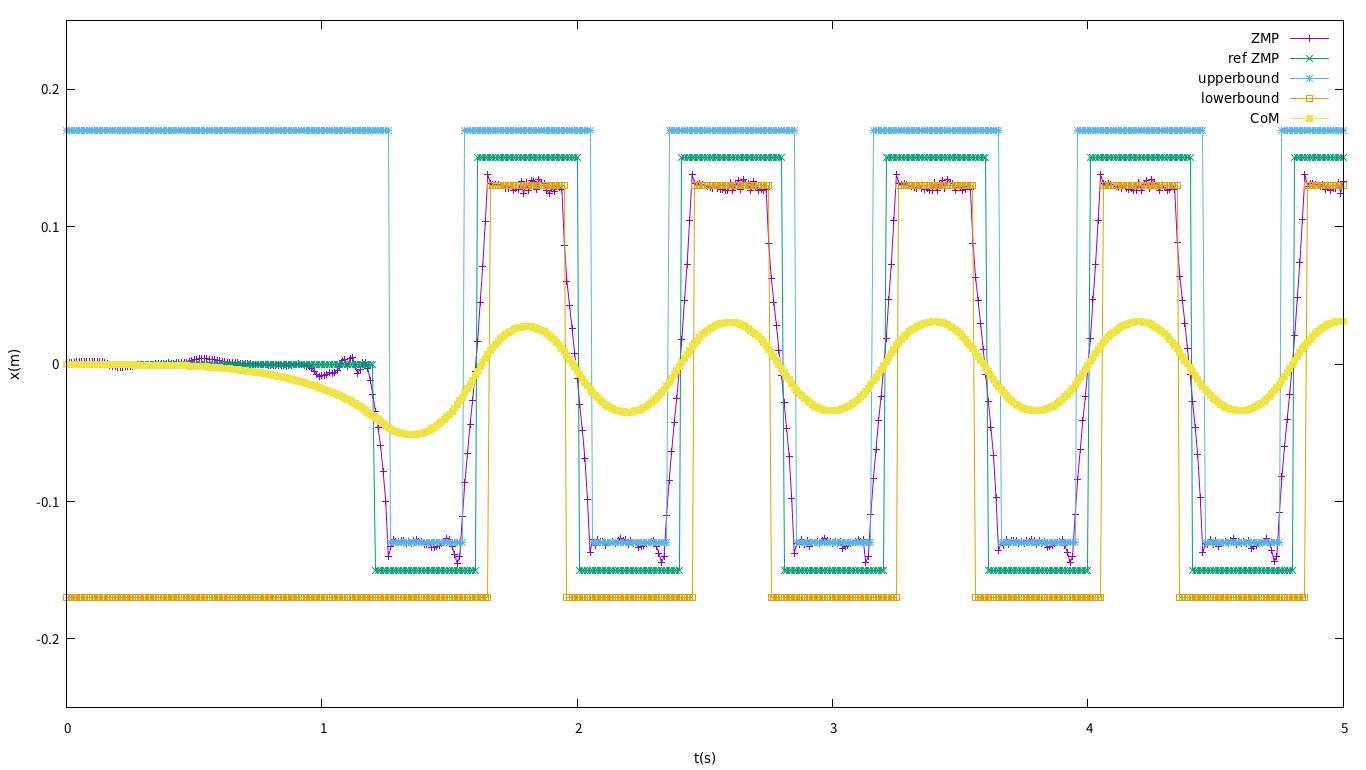
\includegraphics[keepaspectratio, scale=0.25]
      {images/mpc_horizon/mpc_horizon_150.png}
 \caption{Illustration of table-cart model}
 \label{Fig:Illustration of table-cart model}
\end{figure}

\begin{figure}[H]
  \centering
 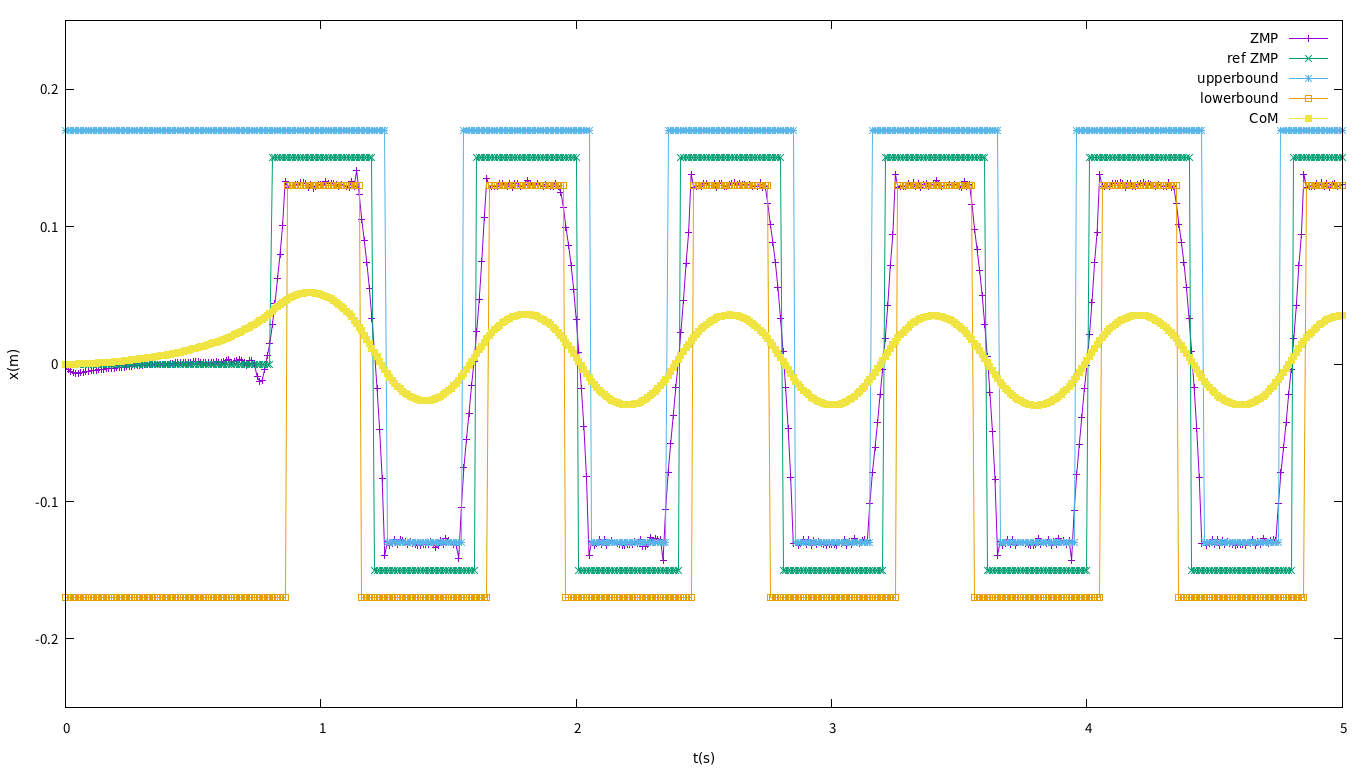
\includegraphics[keepaspectratio, scale=0.25]
      {images/mpc_horizon/mpc_horizon_200.png}
 \caption{Illustration of table-cart model}
 \label{Fig:Illustration of table-cart model}
\end{figure}

\begin{figure}[H]
  \centering
 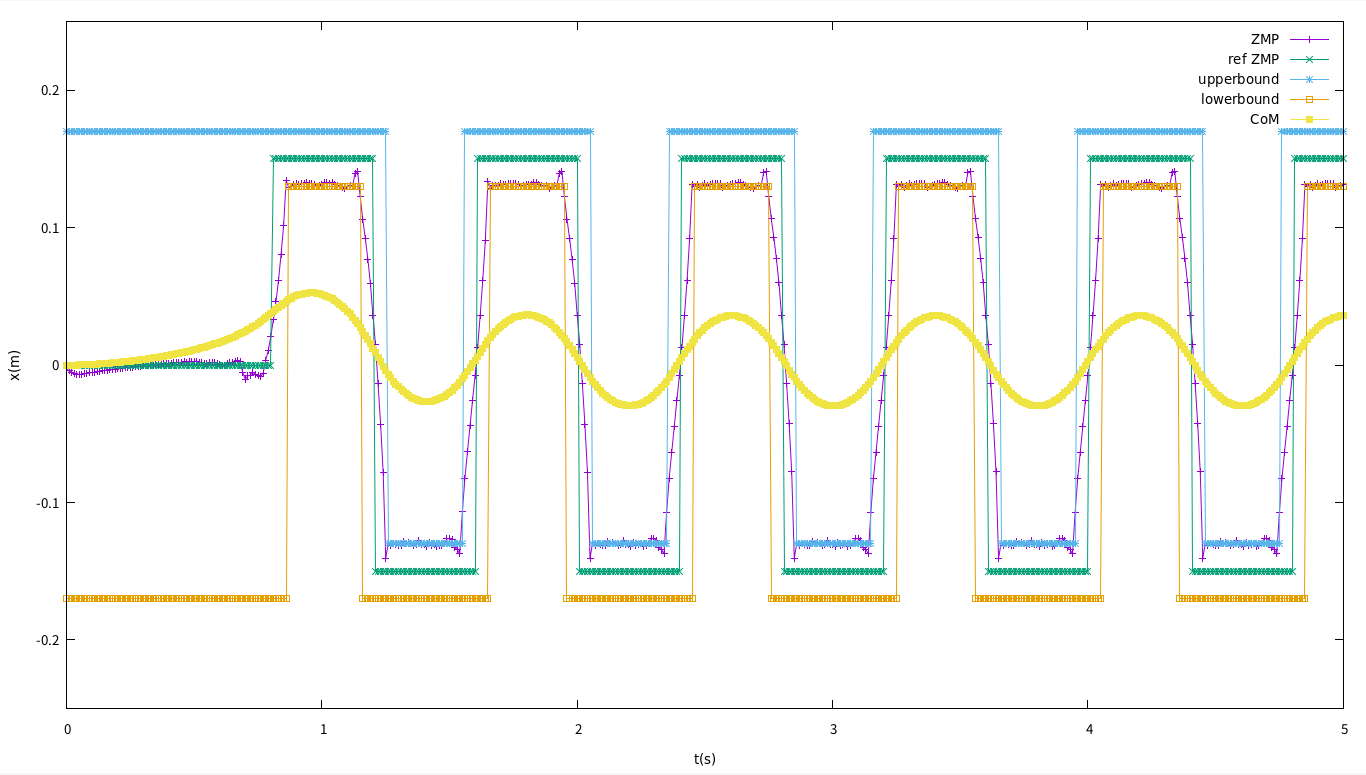
\includegraphics[keepaspectratio, scale=0.25]
      {images/mpc_horizon/mpc_horizon_250.png}
 \caption{Illustration of table-cart model}
 \label{Fig:Illustration of table-cart model}
\end{figure}

\begin{figure}[H]
  \centering
 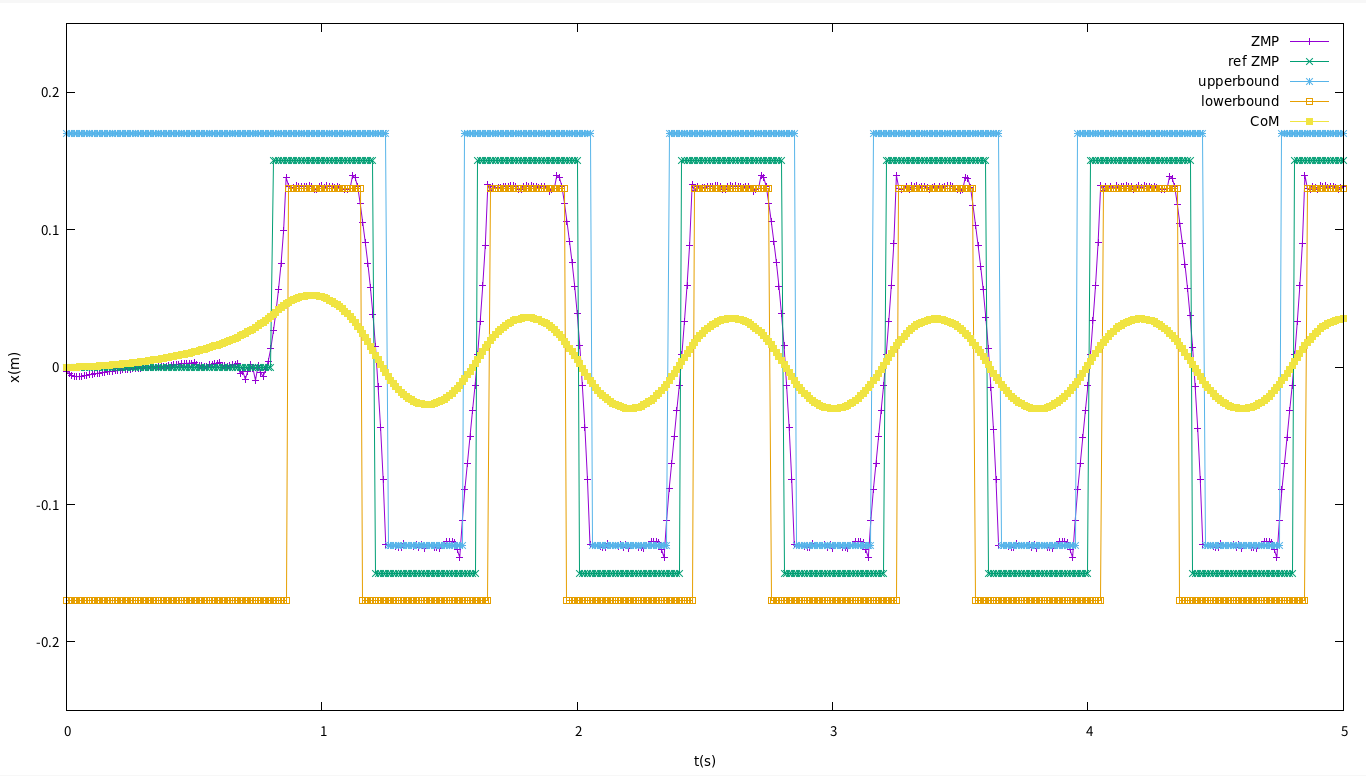
\includegraphics[keepaspectratio, scale=0.25]
      {images/mpc_horizon/mpc_horizon_300.png}
 \caption{Illustration of table-cart model}
 \label{Fig:Illustration of table-cart model}
\end{figure}

%---------------------------------------------------------
\subsection{Q / R}
\begin{figure}[H]
  \centering
 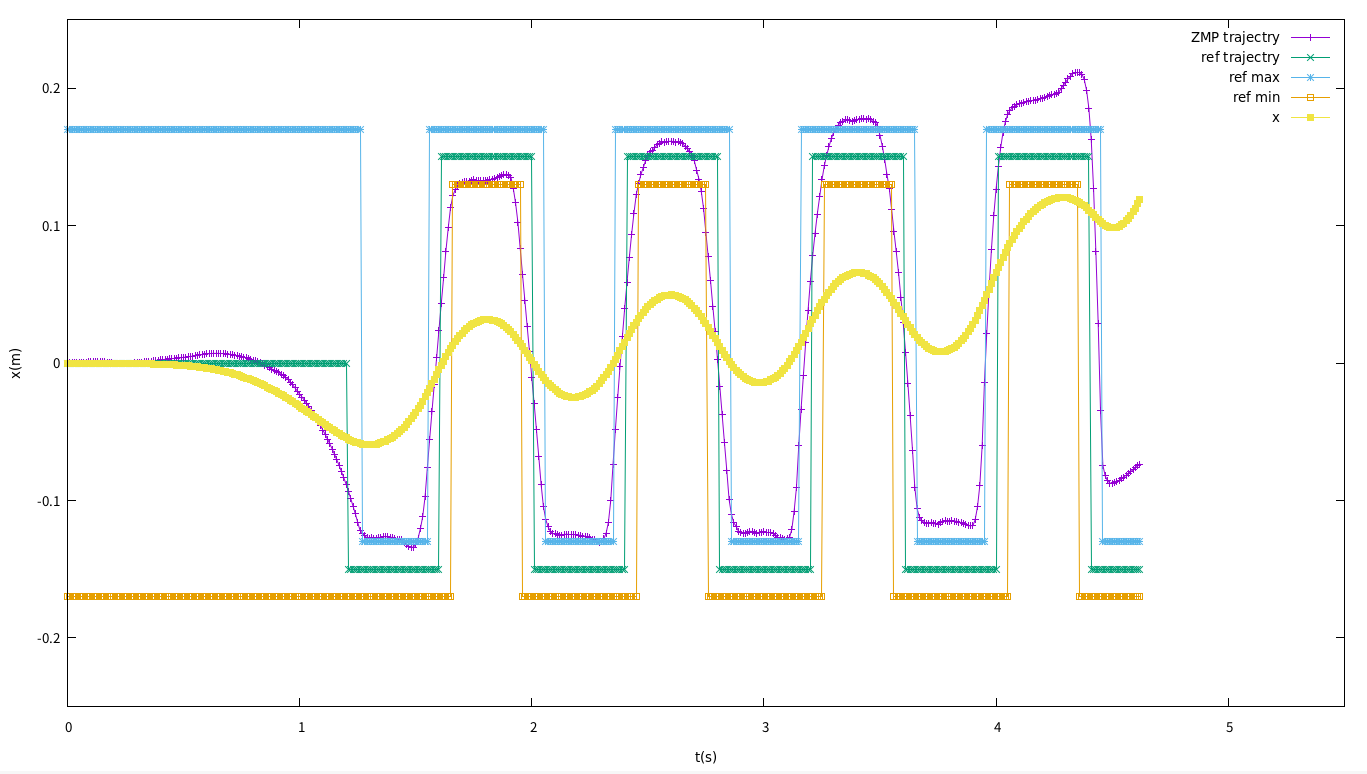
\includegraphics[keepaspectratio, scale=0.25]
      {images/mpc_qr/mpc_qr_10_4_error.png}
 \caption{Illustration of table-cart model}
 \label{Fig:Illustration of table-cart model}
\end{figure}

\begin{figure}[H]
  \centering
 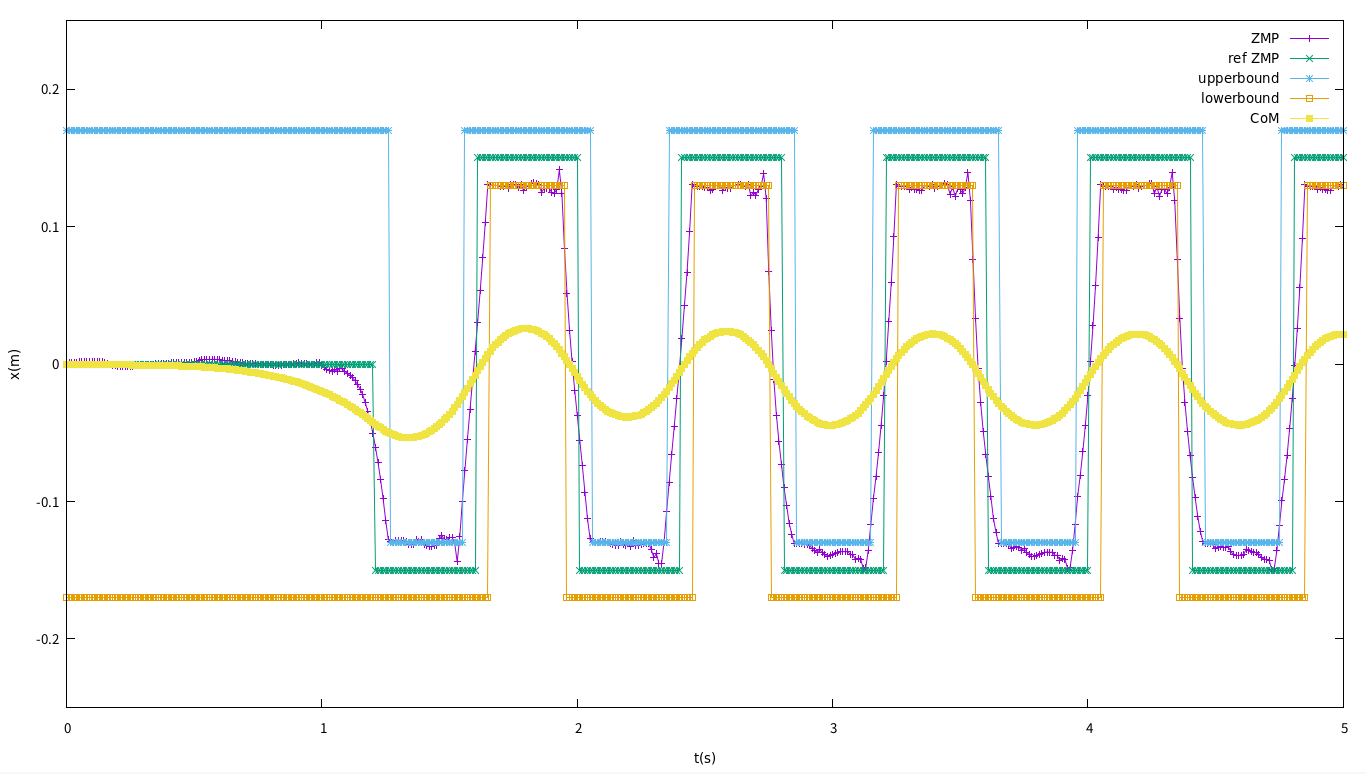
\includegraphics[keepaspectratio, scale=0.25]
      {images/mpc_qr/mpc_qr_10_5.png}
 \caption{Illustration of table-cart model}
 \label{Fig:Illustration of table-cart model}
\end{figure}

\begin{figure}[H]
  \centering
 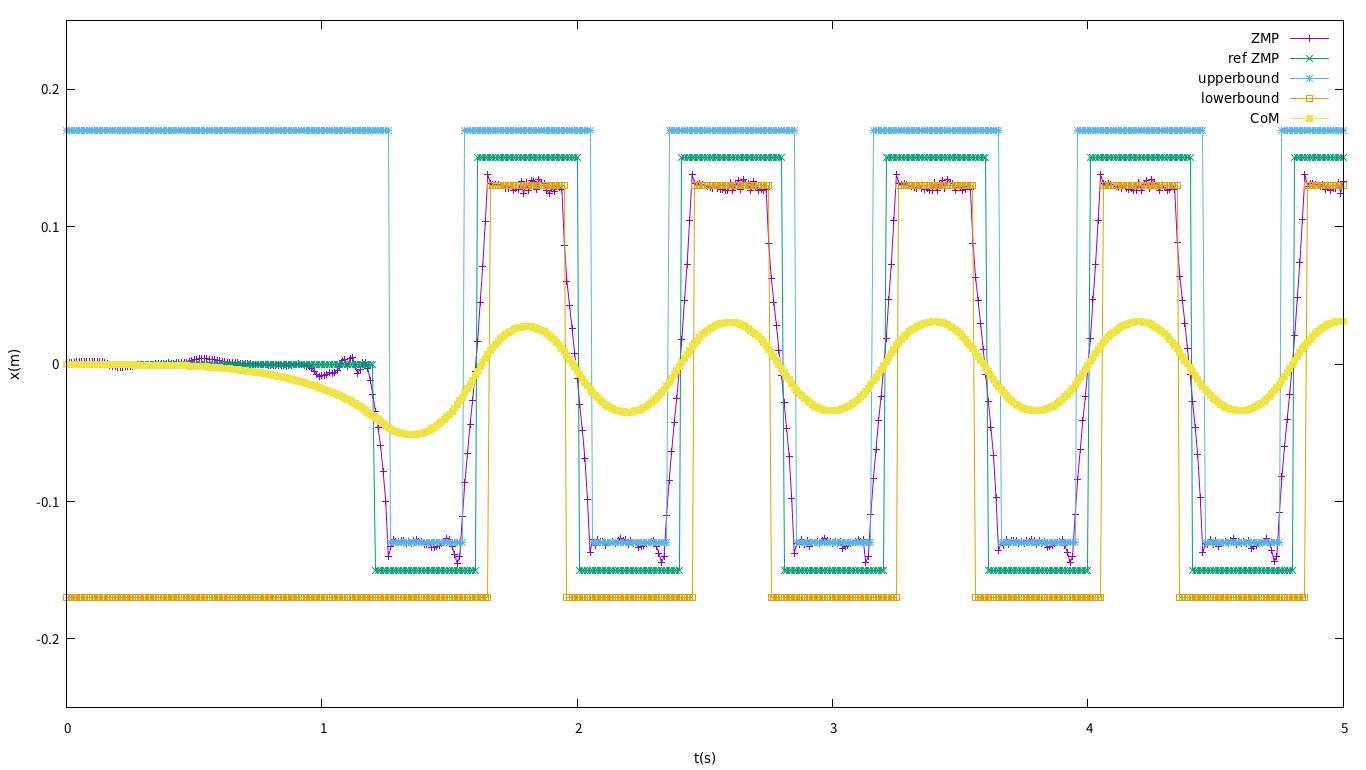
\includegraphics[keepaspectratio, scale=0.25]
      {images/mpc_qr/mpc_qr_10_6.png}
 \caption{Illustration of table-cart model}
 \label{Fig:Illustration of table-cart model}
\end{figure}

\begin{figure}[H]
  \centering
 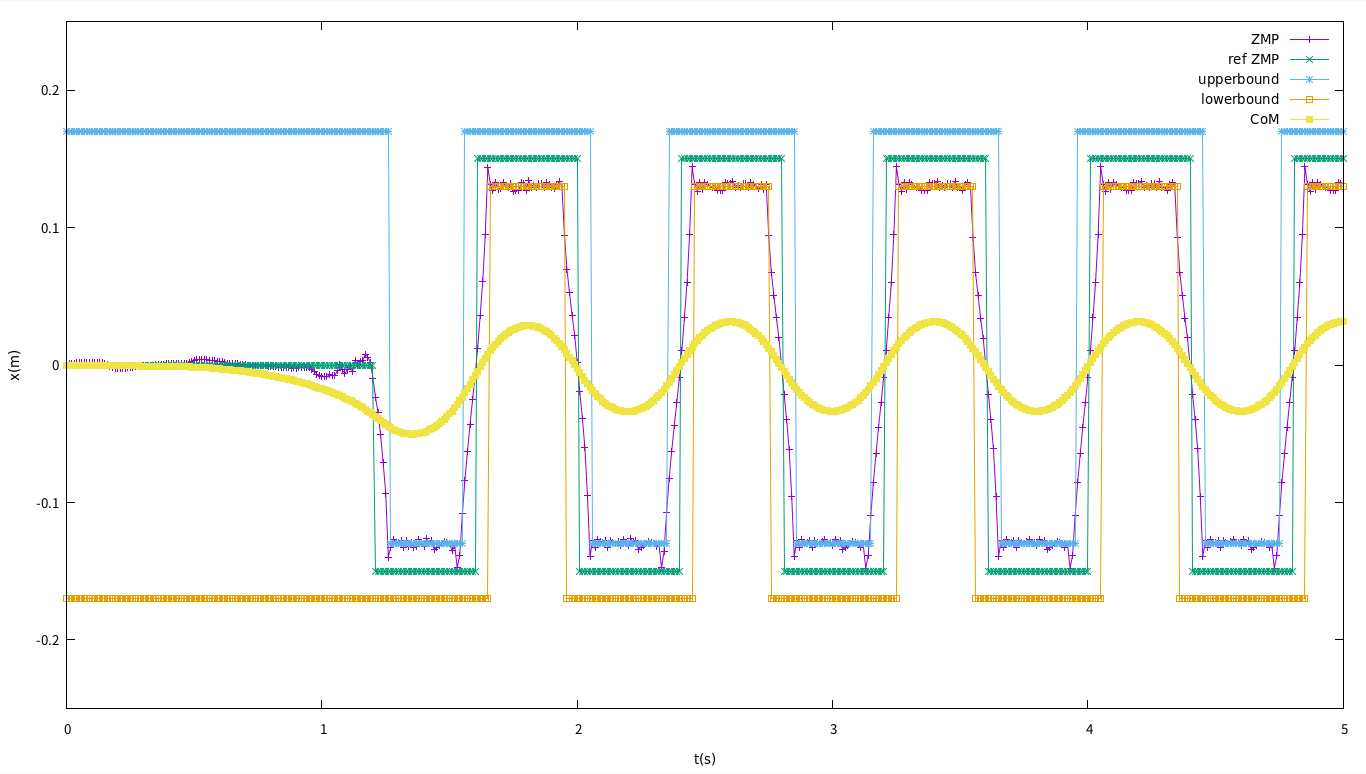
\includegraphics[keepaspectratio, scale=0.25]
      {images/mpc_qr/mpc_qr_10_7.png}
 \caption{Illustration of table-cart model}
 \label{Fig:Illustration of table-cart model}
\end{figure}

\begin{figure}[H]
  \centering
 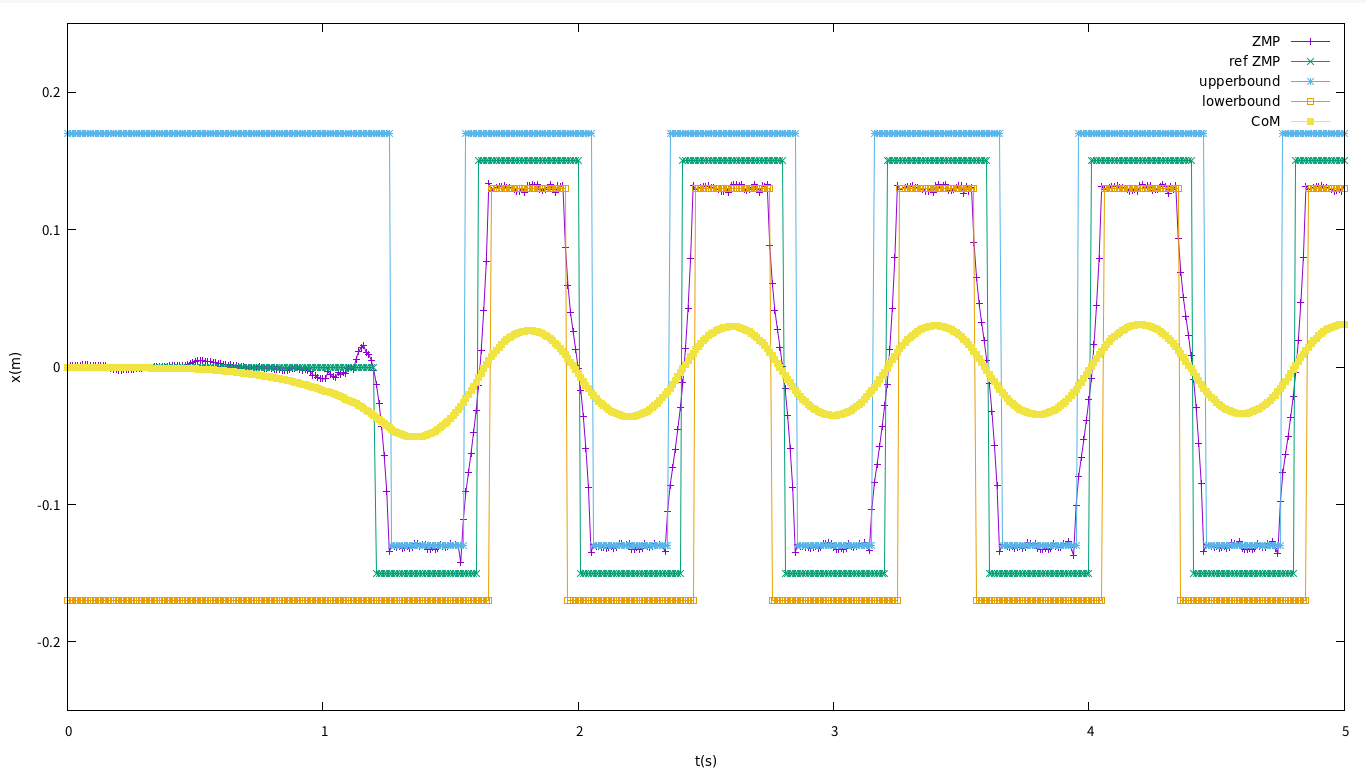
\includegraphics[keepaspectratio, scale=0.25]
      {images/mpc_qr/mpc_qr_10_8.png}
 \caption{Illustration of table-cart model}
 \label{Fig:Illustration of table-cart model}
\end{figure}

\begin{figure}[H]
  \centering
 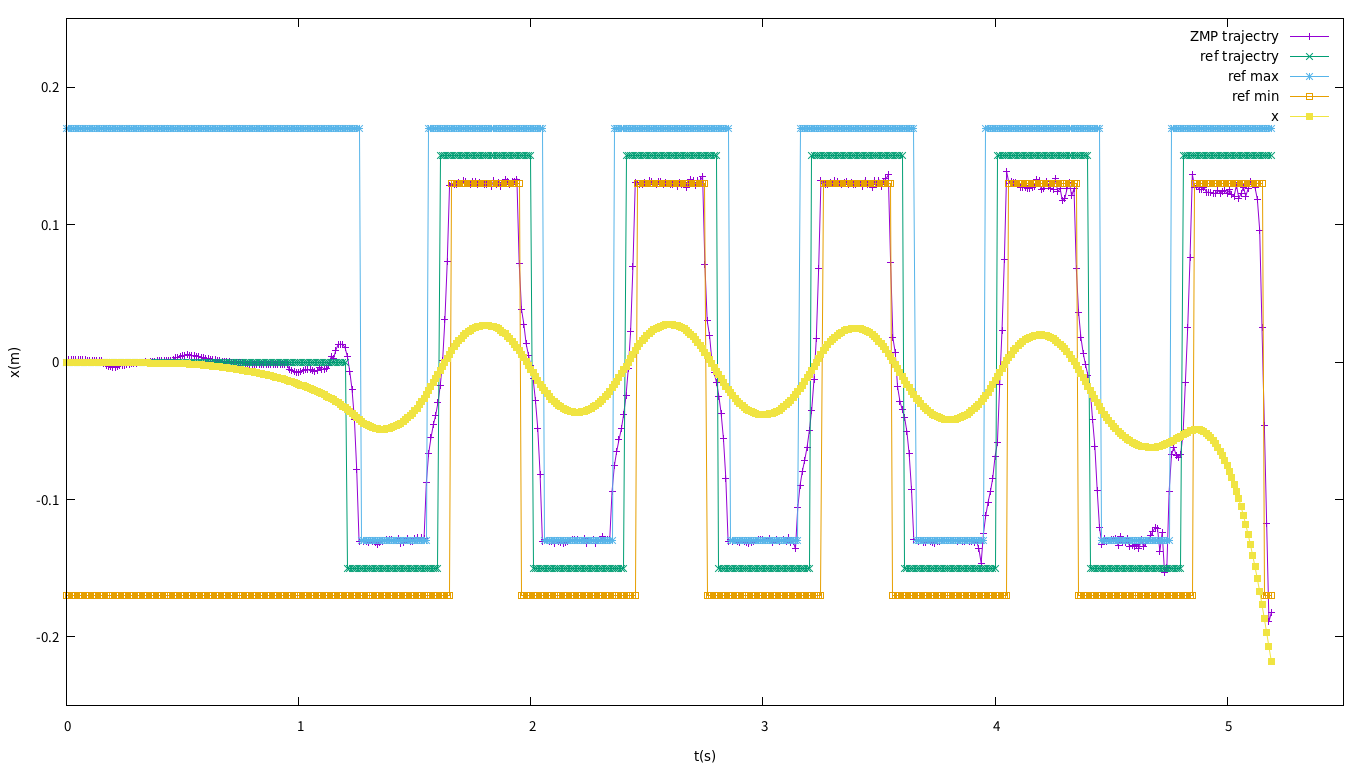
\includegraphics[keepaspectratio, scale=0.25]
      {images/mpc_qr/mpc_qr_10_9_error.png}
 \caption{Illustration of table-cart model}
 \label{Fig:Illustration of table-cart model}
\end{figure}

%-----------------------------------------------------------------
\subsection{start with this step}


\begin{figure}[H]
  \centering
 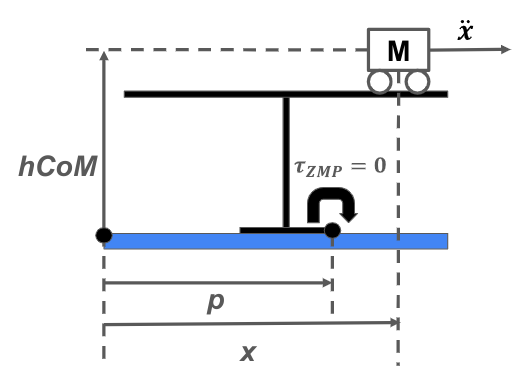
\includegraphics[keepaspectratio, scale=0.5]
      {images/walk/table.png}
 \caption{Illustration of table-cart model}
 \label{Fig:Illustration of table-cart model}
\end{figure}

\newpage
%--------------------------------------------------------
\section{実行時間}
 この節では,4.2で出力したソフトウェアの実行時間を計測する.
計測は各パラメータをそれぞれ10回ずつ行い,平均時間を記録する.表に示す.「x」は生成できていないため対象外とする.
\begin{table}[hbtp]
  \centering
  \caption{Execution time of each Q/R}
  \label{Execution time of each Q/R}
  \begin{tabular}{|l|l|l|l|l|l|l|}
  \hline \hline
  Q / R        & 10\textasciicircum{}4 & 10\textasciicircum{}5 & 10\textasciicircum{}6 & 10\textasciicircum{}7 & 10\textasciicircum{}8 & 10\textasciicircum{}9 \\ \hline
  time {[}s{]} & x                     & 4.2                   & 5.6                   & 5.6                   & 5.1                   & x                     \\ \hline
  \end{tabular}
\end{table}

\begin{table}[hbtp]
  \centering
  \caption{Execution time of each Control Horizon}
  \label{Execution time of each Control}
  \begin{tabular}{|l|l|l|l|l|l|l|}
  \hline \hline
  Control Horizon {[}s{]} & 0.5 & 1.0 & 1.5 & 2.0 & 2.5  & 3.0  \\ \hline
  time {[}s{]}            & x   & 3.7 & 5.6 & 9.5 & 12.2 & 15.0 \\ \hline
  \end{tabular}
\end{table}

%---------------------------------------------------------------------
\section{パラメータの傾向}

 Control Horizon
Q/R
実行時間
%Q/Rの値は$10\textasciicircum{}5$と$10\textasciicircum{}5$の間は1秒の差があるが,その他の値は上げても実行時間に大きな差はなかった.
Control Horizonは最適化問題を解く区間が長くなったため実行時間は比例した.
\newpage
%
%% Back Matter
\backmatter{}
%
\include{backmatter/main}
%

\end{document}
